\section{Hardware}

\begin{figure}[H]
\begin{subfigure}{.45\textwidth}
\centering
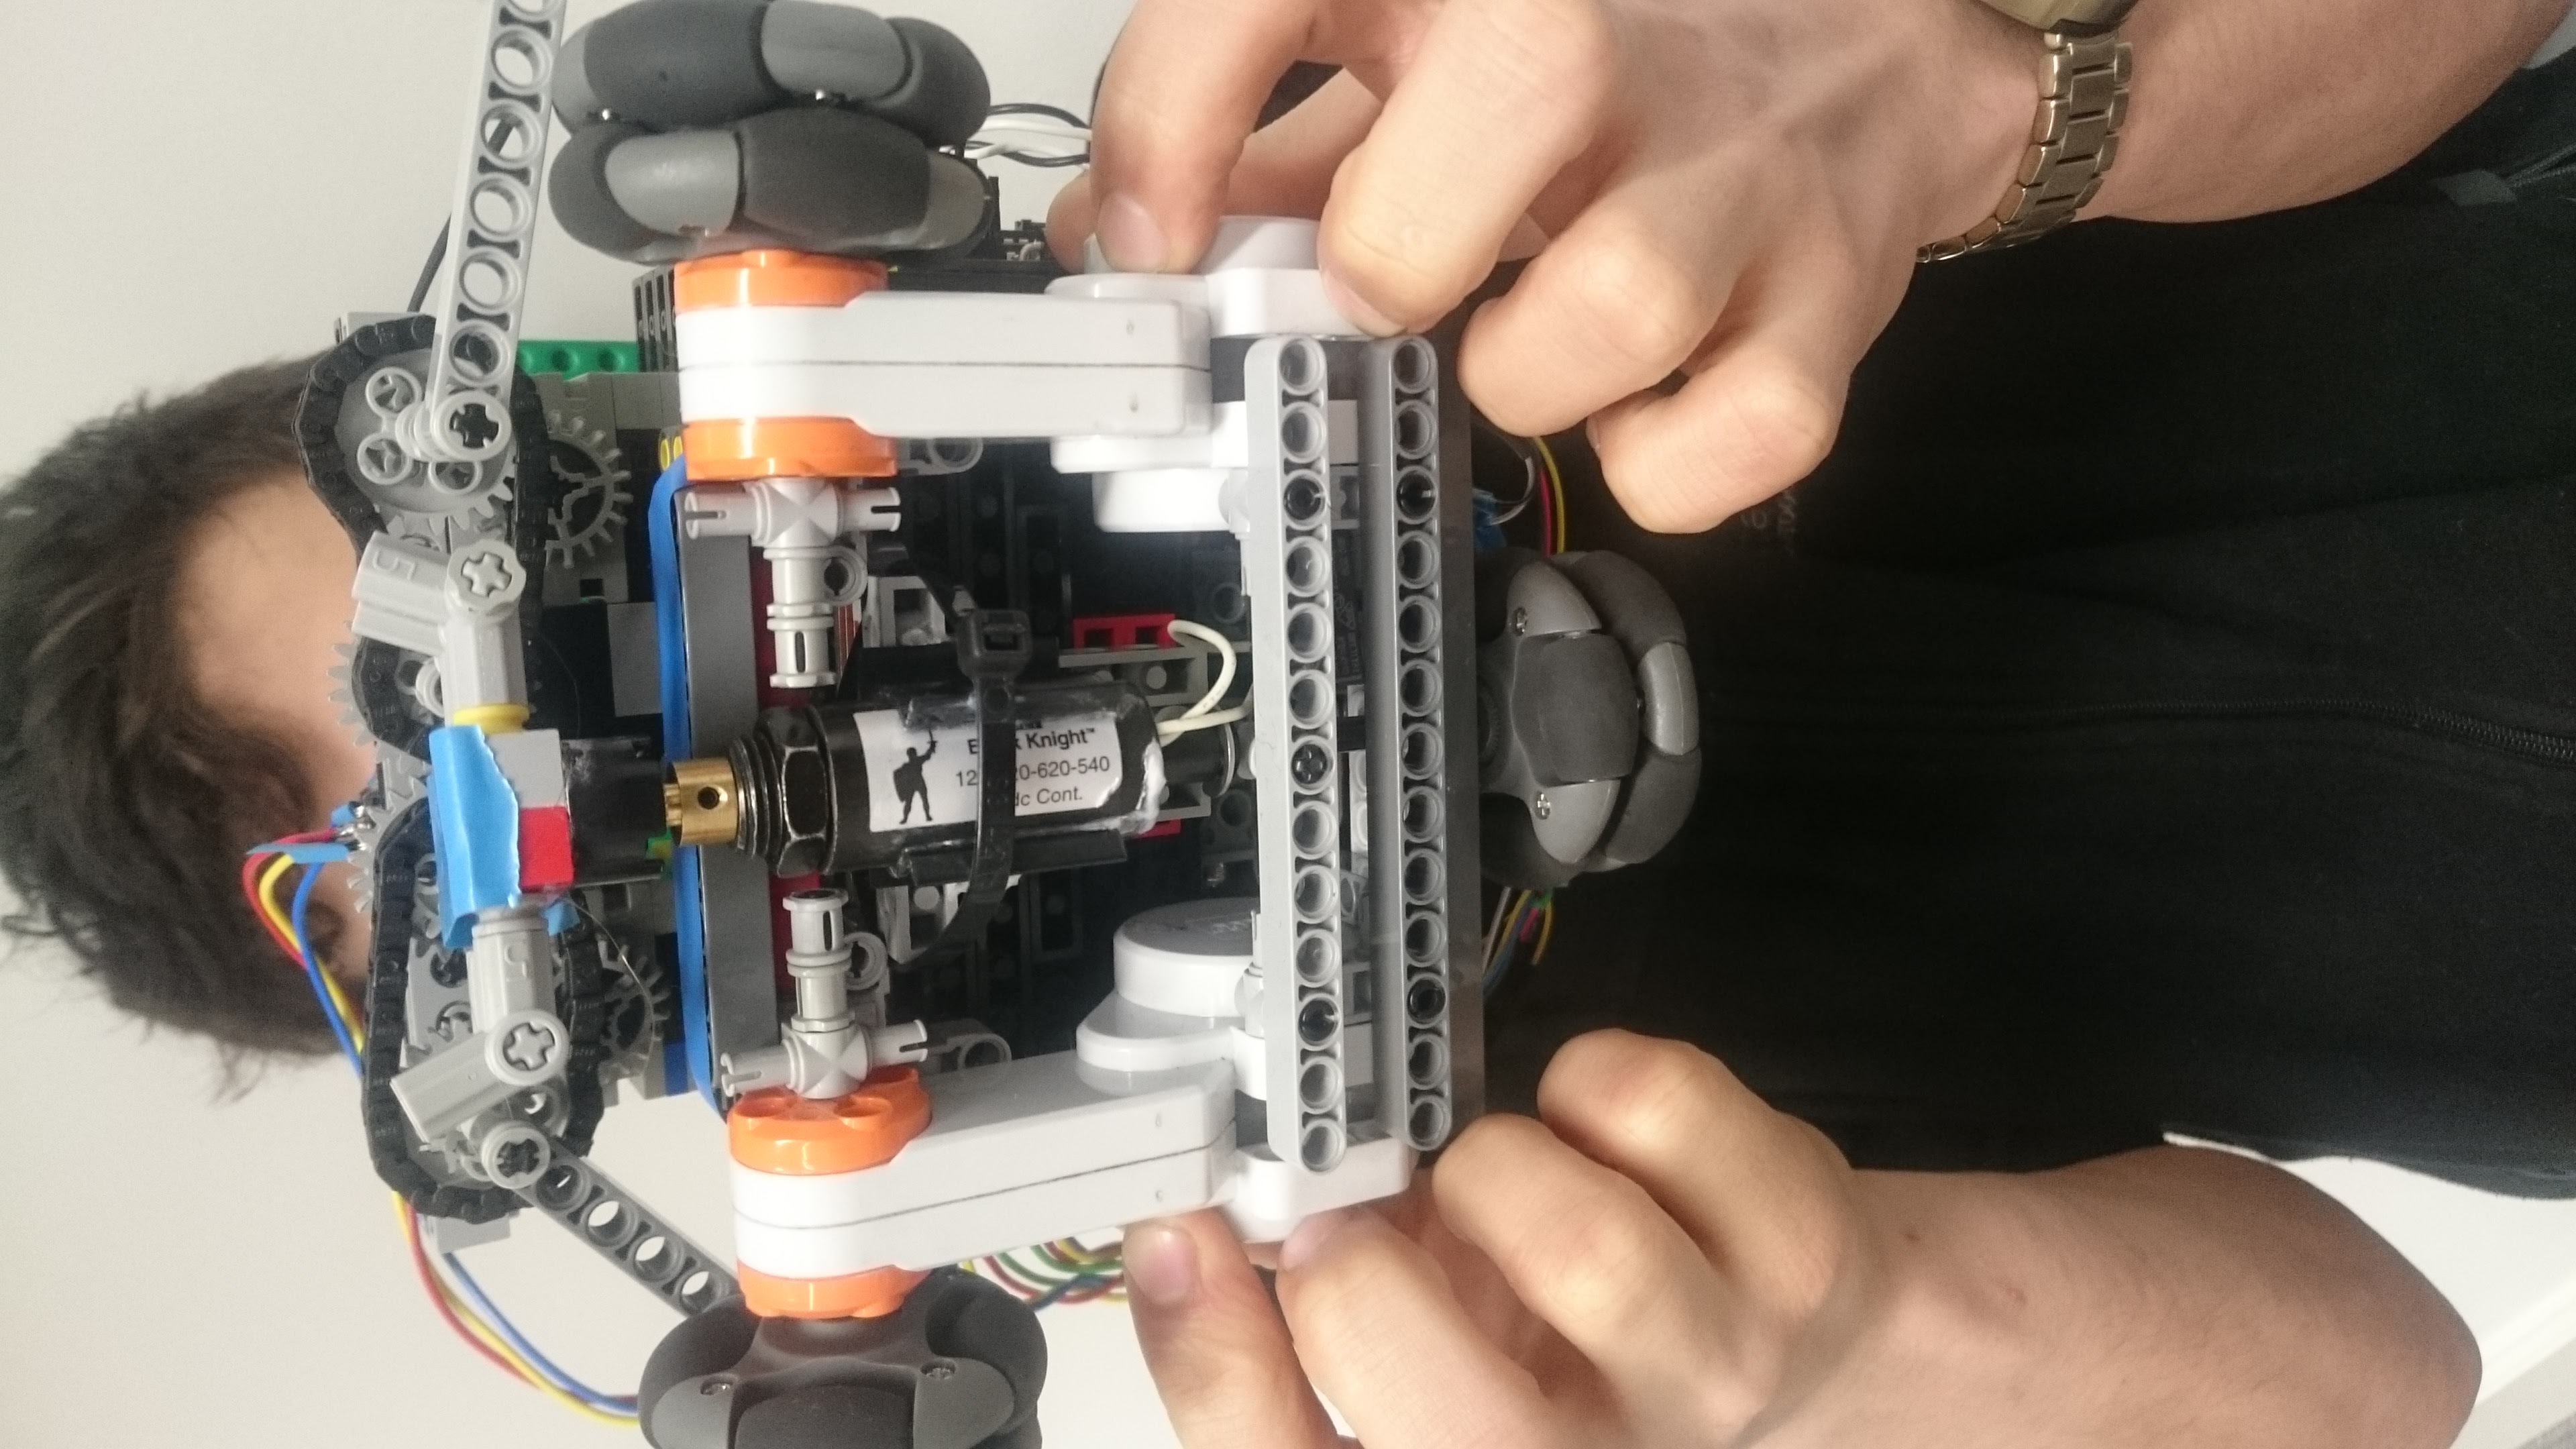
\includegraphics[width=.95\textwidth]{DSC_0036.jpg}
\caption{Wheelbase}
\label{pic:wheelbase}
\end{subfigure}
\begin{subfigure}{.45\textwidth}
\centering
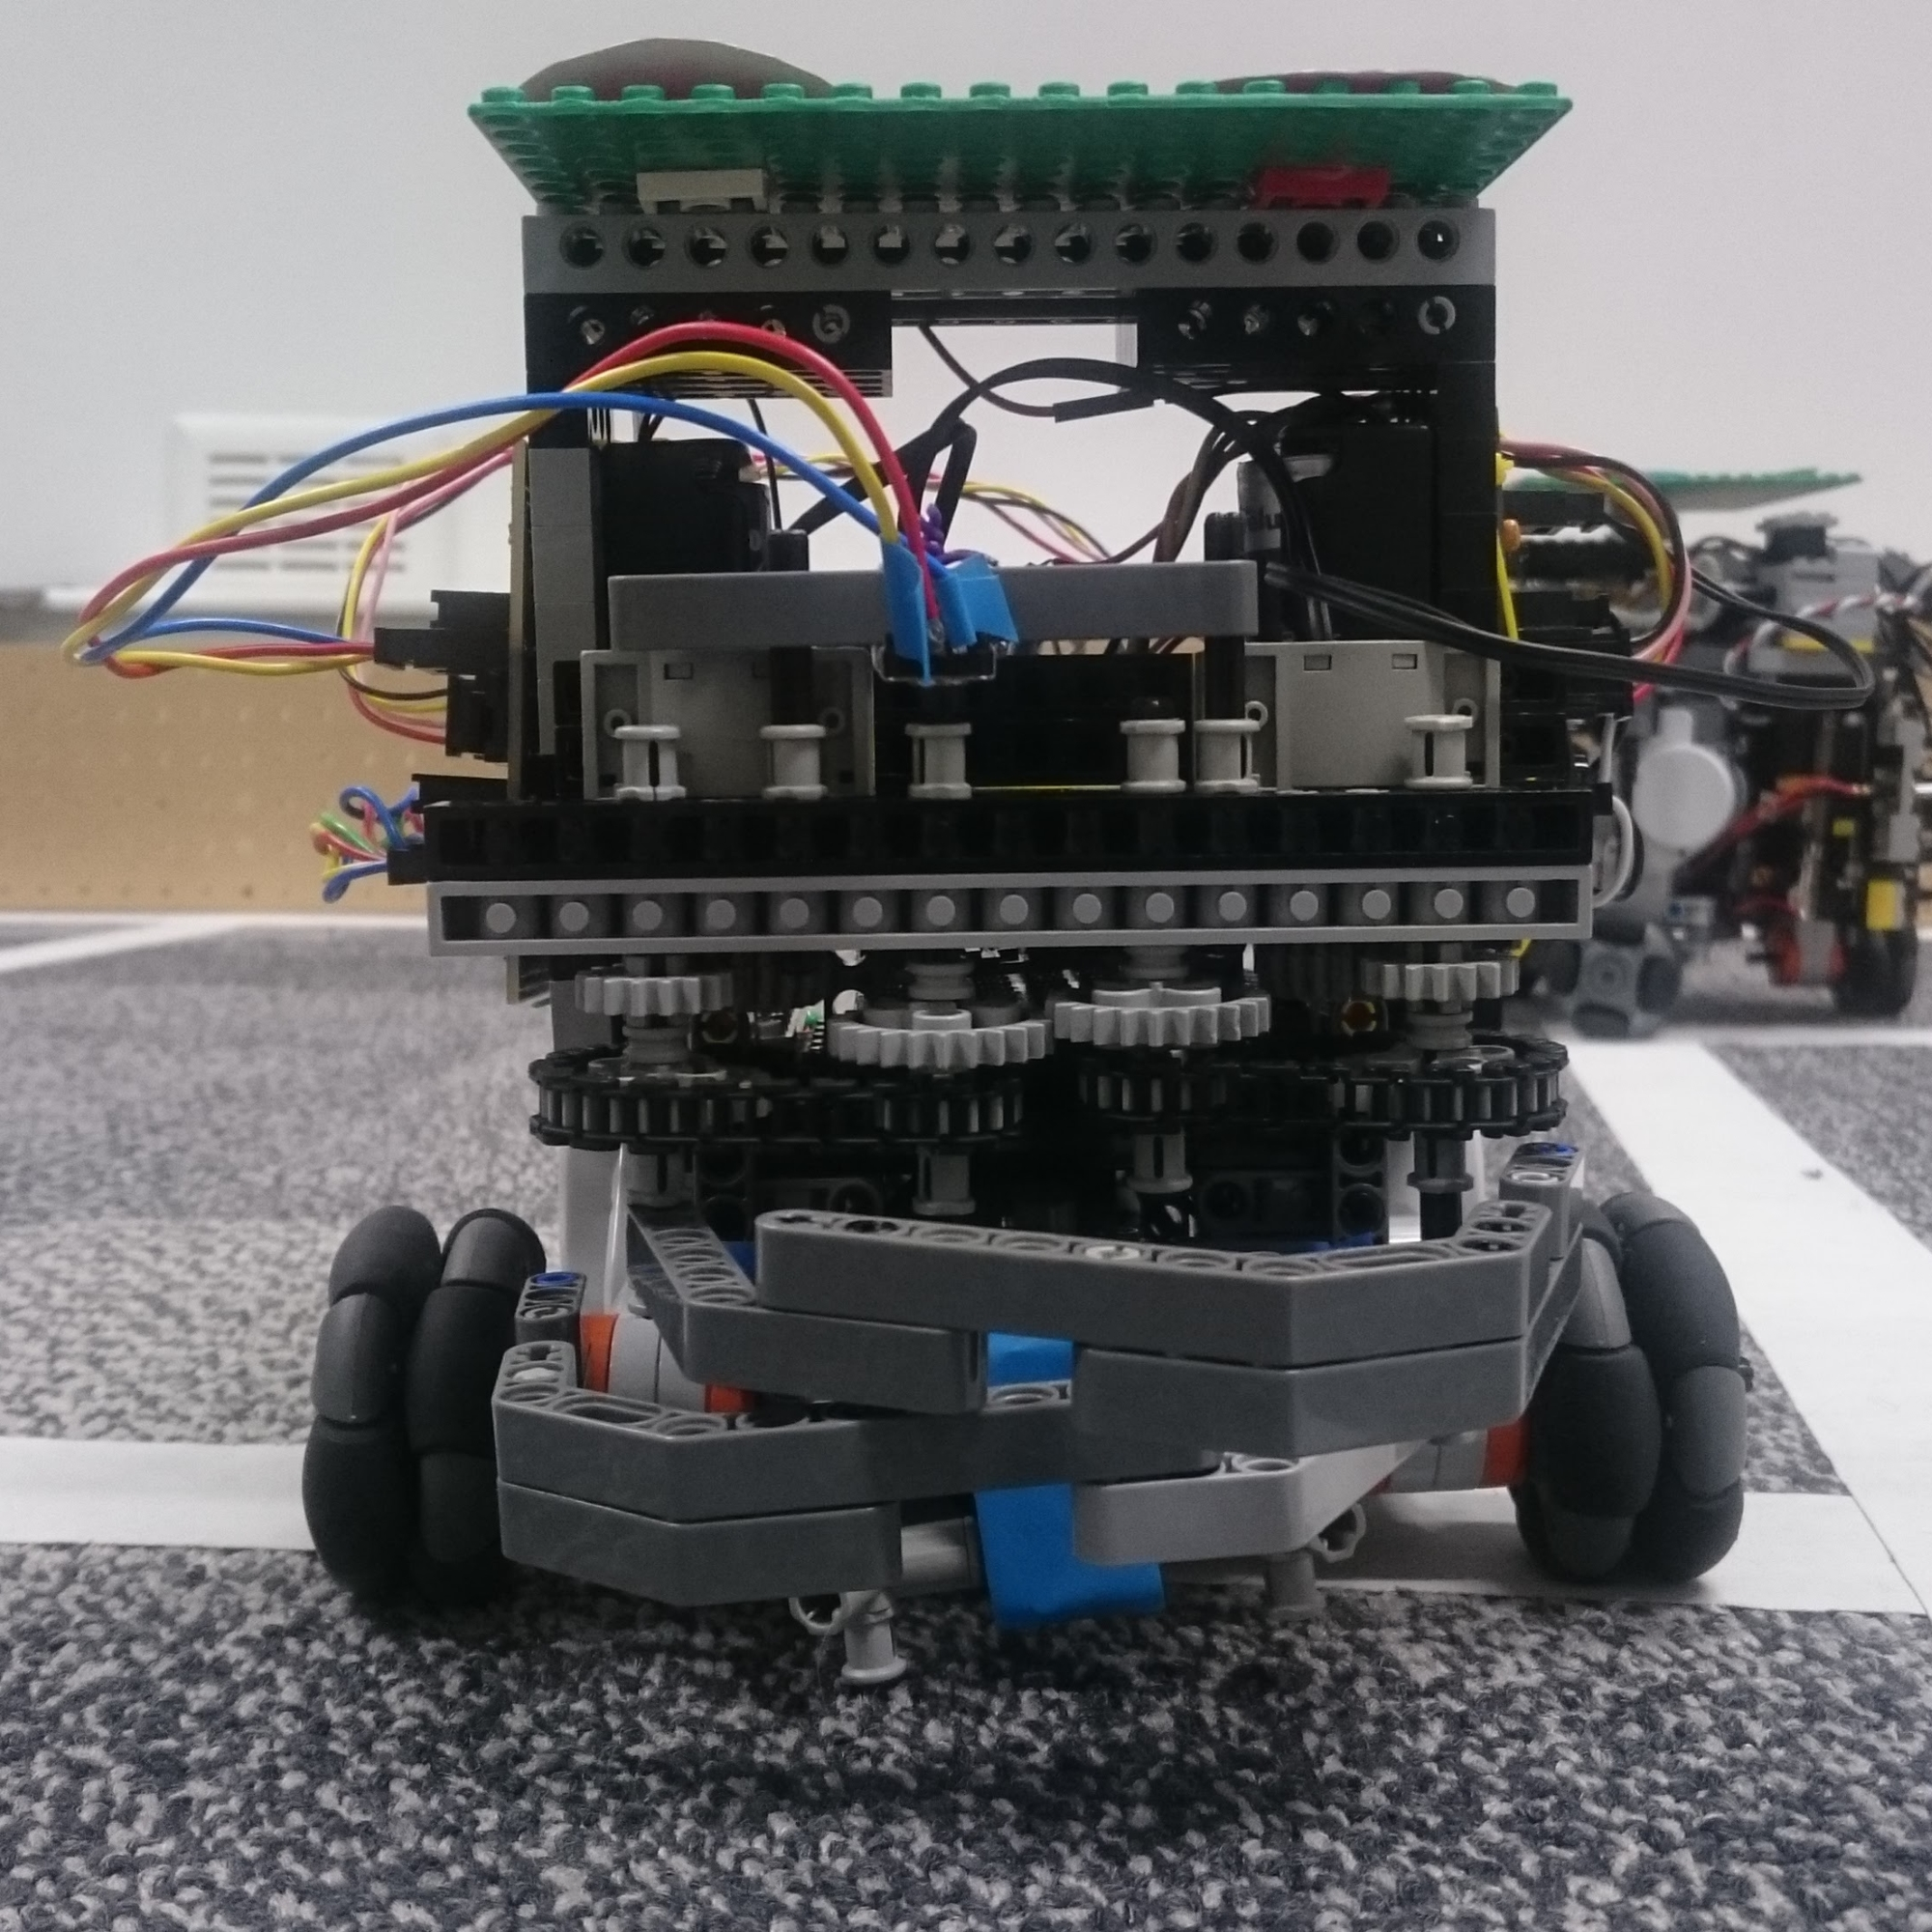
\includegraphics[width=.95\textwidth]{DSC_0031.jpg}
\caption{Front Assembly}
\label{pic:front}
\end{subfigure}
\caption{Robot Construction}
\label{pic:construction}
\end{figure}

\subsection{Wheelbase}
\subsubsection{Dimensions}
'Drive' wheelbase:		15cm \newline
Radius of 'turn' wheel: 11cm
\subsubsection{Origin}
The origin is directly between the 'Drive' wheels
\subsubsection{Arrangement}
The robot uses a 3 wheeled 'T' design with 2 parallel 'drive' wheels along one axis of rotation (capable of rotating independently) and a third unpowered 'turn' wheel rotating perpendicular to these 2 (\autoref{pic:wheelbase}). The 'origin' of the robot should be 
directly between the 2 drive wheels which are 15cm apart. The 'turn' wheel 
is 11cm back from the origin, the left wheel 7.5cm to the left and the right
7.5cm to the right. 

\subsubsection{Motors}
The 2 drive motors are lego NXT motors and have rotational encoders built in, this is used to turn and move accurately. 



\subsection{Front Assembly}
\subsubsection{Description}
The robot Has a 2 motor assembly mounted on 4 vertical bars coming up from the struts joining the left and right NXT drive motors. These are symmetrically mounted and linked by a chain in order to keep them synchronised. The right grabber is lower than the left one so that they do not hit into each other. On one of the centre axles there is a rotary encoder to give the position of the grabbers to the Arduino, through the rotary encoder board. Position 0 is open, 10 is closed with ball and 13 is closed without ball. See \autoref{pic:front}.

The grabber assembly is fully detachable and can be clipped on and off. 


\subsection{Kicker}
\subsubsection{Position}
The kicker is a solenoid mounted on the underside of the robot (see \autoref{pic:construction}) connected through a relay to the battery packs, with the relay signal going to the power shield and being controlled directly by the Arduino. on the end of the solenoid is a curved kicker designed to keep the ball straight.

\subsubsection{Power}
The kicker is capable of kicking a distance of 3.2m at full power with an approx error of 15 percent

\subsection{Board and Battery Assembly}
\subsubsection{Structure}
The boards are mounted on a platform between the 3 wheels. The Arduino and power
shield are mounted in the centre with 2 battery packs of 2 18650 Li-Ion batteries mounted sideways on either
side. The rotary encoder board is
mounted on the back of the right battery pack and the motor driver board is mounted
on the left battery pack. As the batteries face in the packs must be detached to
replace them. Both packs clip onto the platform with lego connectors.

\subsubsection{Batteries}
The batteries are 4* 18650 Canwelum Li-Ion cells wired in series in 2 battery packs. They can be removed and charged individually in the Li-Ion charger.

\begin{table}[H]
\begin{tabularx}{\textwidth}{XX}
\textbf{Voltage (per cell):}	& 2.65 - 4.2 \\
\textbf{Voltage (total):}		& 10.6 - 16.8 \\
\textbf{Max Current:}			& 7A \\
\textbf{Internal Resistance (per cell)}: & 0.150 Ohms \\
\textbf{Internal Resistance (total)}: & 0.6 Ohms \\
\textbf{Capacity}: & 2250mAh \\
\textbf{Protection}: & overvolt and undervolt \\
\end{tabularx}
\end{table}
   
\subsubsection{Connections}
The batteries are connected in series and must be connected to the power board through the yellow switch, with the splitters on the line powering the solenoid relay (orange wires)
\subsubsection{Switch}
A yellow switch turns the robot on and off